% Options for packages loaded elsewhere
\PassOptionsToPackage{unicode}{hyperref}
\PassOptionsToPackage{hyphens}{url}
%
\documentclass[
]{book}
\usepackage{lmodern}
\usepackage{amssymb,amsmath}
\usepackage{ifxetex,ifluatex}
\ifnum 0\ifxetex 1\fi\ifluatex 1\fi=0 % if pdftex
  \usepackage[T1]{fontenc}
  \usepackage[utf8]{inputenc}
  \usepackage{textcomp} % provide euro and other symbols
\else % if luatex or xetex
  \usepackage{unicode-math}
  \defaultfontfeatures{Scale=MatchLowercase}
  \defaultfontfeatures[\rmfamily]{Ligatures=TeX,Scale=1}
\fi
% Use upquote if available, for straight quotes in verbatim environments
\IfFileExists{upquote.sty}{\usepackage{upquote}}{}
\IfFileExists{microtype.sty}{% use microtype if available
  \usepackage[]{microtype}
  \UseMicrotypeSet[protrusion]{basicmath} % disable protrusion for tt fonts
}{}
\makeatletter
\@ifundefined{KOMAClassName}{% if non-KOMA class
  \IfFileExists{parskip.sty}{%
    \usepackage{parskip}
  }{% else
    \setlength{\parindent}{0pt}
    \setlength{\parskip}{6pt plus 2pt minus 1pt}}
}{% if KOMA class
  \KOMAoptions{parskip=half}}
\makeatother
\usepackage{xcolor}
\IfFileExists{xurl.sty}{\usepackage{xurl}}{} % add URL line breaks if available
\IfFileExists{bookmark.sty}{\usepackage{bookmark}}{\usepackage{hyperref}}
\hypersetup{
  pdftitle={Working Title: the data science canon},
  pdfauthor={Databrew},
  hidelinks,
  pdfcreator={LaTeX via pandoc}}
\urlstyle{same} % disable monospaced font for URLs
\usepackage{longtable,booktabs}
% Correct order of tables after \paragraph or \subparagraph
\usepackage{etoolbox}
\makeatletter
\patchcmd\longtable{\par}{\if@noskipsec\mbox{}\fi\par}{}{}
\makeatother
% Allow footnotes in longtable head/foot
\IfFileExists{footnotehyper.sty}{\usepackage{footnotehyper}}{\usepackage{footnote}}
\makesavenoteenv{longtable}
\usepackage{graphicx,grffile}
\makeatletter
\def\maxwidth{\ifdim\Gin@nat@width>\linewidth\linewidth\else\Gin@nat@width\fi}
\def\maxheight{\ifdim\Gin@nat@height>\textheight\textheight\else\Gin@nat@height\fi}
\makeatother
% Scale images if necessary, so that they will not overflow the page
% margins by default, and it is still possible to overwrite the defaults
% using explicit options in \includegraphics[width, height, ...]{}
\setkeys{Gin}{width=\maxwidth,height=\maxheight,keepaspectratio}
% Set default figure placement to htbp
\makeatletter
\def\fps@figure{htbp}
\makeatother
\setlength{\emergencystretch}{3em} % prevent overfull lines
\providecommand{\tightlist}{%
  \setlength{\itemsep}{0pt}\setlength{\parskip}{0pt}}
\setcounter{secnumdepth}{5}
\usepackage{booktabs}
\usepackage{amsthm}
\makeatletter
\def\thm@space@setup{%
  \thm@preskip=8pt plus 2pt minus 4pt
  \thm@postskip=\thm@preskip
}
\makeatother
\usepackage[]{natbib}
\bibliographystyle{apalike}

\title{Working Title: the data science canon}
\author{Databrew}
\date{2021-03-27}

\begin{document}
\maketitle

{
\setcounter{tocdepth}{1}
\tableofcontents
}
\hypertarget{welcome}{%
\chapter{Welcome}\label{welcome}}

Welcome to \emph{Working Title}, the data science canon by \emph{DataBrew}

\hypertarget{part-core-theory}{%
\part{Core theory}\label{part-core-theory}}

\hypertarget{principles-of-data-science}{%
\chapter{Principles of data science}\label{principles-of-data-science}}

\hypertarget{what-is-data-science}{%
\section{What is data science?}\label{what-is-data-science}}

\hypertarget{what-is-the-data-life-cycle}{%
\section{What is the data life cycle?}\label{what-is-the-data-life-cycle}}

\hypertarget{what-is-a-pipeline}{%
\section{What is a pipeline?}\label{what-is-a-pipeline}}

\hypertarget{data-science-in-the-wild}{%
\section{Data science `in the wild'}\label{data-science-in-the-wild}}

\hypertarget{the-reproducibility-crisis}{%
\section{The reproducibility crisis}\label{the-reproducibility-crisis}}

\hypertarget{visualizing-data}{%
\chapter{Visualizing data}\label{visualizing-data}}

\hypertarget{bad-examples}{%
\section{Bad examples}\label{bad-examples}}

\hypertarget{good-exaples}{%
\section{Good exaples}\label{good-exaples}}

\hypertarget{edward-tufte}{%
\section{Edward Tufte}\label{edward-tufte}}

\hypertarget{grammar-of-graphics}{%
\section{Grammar of graphics}\label{grammar-of-graphics}}

\hypertarget{design-principles}{%
\section{Design principles}\label{design-principles}}

\hypertarget{plots-power}{%
\section{Plots \& power}\label{plots-power}}

The politics of graphics

\hypertarget{writing-about-data}{%
\chapter{Writing about data}\label{writing-about-data}}

\hypertarget{data-ethics}{%
\chapter{Data ethics}\label{data-ethics}}

\hypertarget{part-getting-started}{%
\part{Getting started}\label{part-getting-started}}

\hypertarget{setting-up-rstudio}{%
\chapter{Setting up RStudio}\label{setting-up-rstudio}}

\hypertarget{running-r-code}{%
\chapter{Running R code}\label{running-r-code}}

\hypertarget{basic-math}{%
\section{Basic math}\label{basic-math}}

\hypertarget{operators}{%
\section{Operators}\label{operators}}

\hypertarget{rstudio-workflows}{%
\chapter{RStudio workflows}\label{rstudio-workflows}}

\hypertarget{tour-of-rstudio}{%
\section{Tour of RStudio}\label{tour-of-rstudio}}

\hypertarget{scripts}{%
\section{Scripts}\label{scripts}}

\hypertarget{typical-workflows}{%
\section{Typical workflows}\label{typical-workflows}}

\hypertarget{objects-in-r}{%
\chapter{Objects in R}\label{objects-in-r}}

\hypertarget{variables}{%
\section{Variables}\label{variables}}

\hypertarget{vectors}{%
\section{Vectors}\label{vectors}}

\hypertarget{calling-functions}{%
\chapter{Calling functions}\label{calling-functions}}

\hypertarget{base-plots}{%
\chapter{Base plots}\label{base-plots}}

\hypertarget{packages}{%
\chapter{Packages}\label{packages}}

\hypertarget{basics-of-ggplot}{%
\chapter{Basics of ggplot}\label{basics-of-ggplot}}

\hypertarget{part-working-with-data-in-r}{%
\part{Working with data in R}\label{part-working-with-data-in-r}}

\hypertarget{importing-data}{%
\chapter{Importing data}\label{importing-data}}

\hypertarget{working-directories}{%
\section{Working directories}\label{working-directories}}

\hypertarget{reading-in-data}{%
\section{Reading in data}\label{reading-in-data}}

\hypertarget{dataframes}{%
\chapter{Dataframes}\label{dataframes}}

\hypertarget{exploration}{%
\section{Exploration}\label{exploration}}

\hypertarget{summarization}{%
\section{Summarization}\label{summarization}}

\hypertarget{data-wrangling}{%
\chapter{Data wrangling}\label{data-wrangling}}

\hypertarget{data-transformation}{%
\section{Data transformation}\label{data-transformation}}

\hypertarget{filtering}{%
\subsection{Filtering}\label{filtering}}

\hypertarget{grouping}{%
\subsection{Grouping}\label{grouping}}

\hypertarget{joining}{%
\subsection{Joining}\label{joining}}

\hypertarget{the-tidyverse-and-tibbles}{%
\section{The tidyverse and tibbles}\label{the-tidyverse-and-tibbles}}

\hypertarget{transformation-with-dplyr}{%
\section{Transformation with dplyr}\label{transformation-with-dplyr}}

\hypertarget{filtering-1}{%
\subsection{Filtering}\label{filtering-1}}

\hypertarget{grouping-1}{%
\subsection{Grouping}\label{grouping-1}}

\hypertarget{mutating}{%
\subsection{Mutating}\label{mutating}}

\hypertarget{part-exploring-analyzing-data}{%
\part{Exploring \& analyzing data}\label{part-exploring-analyzing-data}}

\hypertarget{exploratory-data-analysis}{%
\chapter{Exploratory Data Analysis}\label{exploratory-data-analysis}}

\hypertarget{exploring-distributions}{%
\section{Exploring distributions}\label{exploring-distributions}}

\hypertarget{variable-types-statistics}{%
\section{Variable types \& statistics}\label{variable-types-statistics}}

\hypertarget{descriptive-statistics}{%
\section{Descriptive statistics}\label{descriptive-statistics}}

\hypertarget{significance-statistics}{%
\chapter{Significance statistics}\label{significance-statistics}}

\hypertarget{thinking-about-significance}{%
\section{Thinking about significance}\label{thinking-about-significance}}

\hypertarget{comparison-tests}{%
\section{Comparison tests}\label{comparison-tests}}

\hypertarget{correlation-tests}{%
\section{Correlation tests}\label{correlation-tests}}

\hypertarget{displaying-data}{%
\chapter{Displaying data}\label{displaying-data}}

\hypertarget{tables}{%
\section{Tables}\label{tables}}

\hypertarget{base-plots-1}{%
\section{Base plots}\label{base-plots-1}}

Advanced techniques

\hypertarget{ggplot}{%
\section{ggplot}\label{ggplot}}

Advanced techniques

\hypertarget{part-creating-your-own-dataset}{%
\part{Creating your own dataset}\label{part-creating-your-own-dataset}}

\hypertarget{managing-project-files}{%
\chapter{Managing project files}\label{managing-project-files}}

\hypertarget{formatting-your-own-data}{%
\chapter{Formatting your own data}\label{formatting-your-own-data}}

\hypertarget{reading-excel-files}{%
\chapter{Reading Excel files}\label{reading-excel-files}}

\hypertarget{reading-googlesheets}{%
\chapter{Reading GoogleSheets}\label{reading-googlesheets}}

\hypertarget{reading-online-data}{%
\chapter{Reading online data}\label{reading-online-data}}

\hypertarget{part-your-r-tool-bag}{%
\part{Your R tool bag}\label{part-your-r-tool-bag}}

\hypertarget{joining-datasets}{%
\chapter{Joining datasets}\label{joining-datasets}}

\hypertarget{for-loops}{%
\chapter{\texorpdfstring{\texttt{for} loops}{for loops}}\label{for-loops}}

\hypertarget{learning-goals}{%
\section*{Learning goals}\label{learning-goals}}
\addcontentsline{toc}{section}{Learning goals}

\begin{itemize}
\tightlist
\item
  What \texttt{for} loops are, and how to use them yourself
\item
  How to use \texttt{for} loops for multi-pane plotting\\
\item
  How to use \texttt{for} loops to achieve complex plots\\
\item
  How to use \texttt{for} loops to summarize data efficiently
\end{itemize}

\hypertarget{coming-soon}{%
\section*{Coming soon}\label{coming-soon}}
\addcontentsline{toc}{section}{Coming soon}

\begin{itemize}
\tightlist
\item
  Instructor notes and answer keys (hidden from students)
\end{itemize}

\hypertarget{tutorial-video}{%
\section*{Tutorial video}\label{tutorial-video}}
\addcontentsline{toc}{section}{Tutorial video}

\emph{(coming soon!)}

\hypertarget{basics}{%
\section*{Basics}\label{basics}}
\addcontentsline{toc}{section}{Basics}

A \texttt{for} loop is a super powerful coding tool. In a \texttt{for} loop, \texttt{R} loops through a chunk of code for a set number of repititions.

A super basic example:

\begin{verbatim}
[1] 1
[1] 2
[1] 3
[1] 4
[1] 5
\end{verbatim}

Here's an example of a pretty useless \texttt{for} loop:

\begin{verbatim}
[1] "I'm just repeating myself."
[1] "I'm just repeating myself."
[1] "I'm just repeating myself."
[1] "I'm just repeating myself."
[1] "I'm just repeating myself."
\end{verbatim}

\textbf{This code is saying:}\\
- For each iteration of this loop, step to the next value in \texttt{x} (first example) or \texttt{1:5} (second example).\\
- Store that value in an object \texttt{i},\\
- and run the code inside the curly brackets.
- Repeat until the end of \texttt{x}.

\textbf{Look at the basic structure:}\\
- In the\texttt{for(\ )} parenthetical, you tell R what values to step through (\texttt{x}), and how to refer to the value in each iteration (\texttt{i}).\\
- Within the curly brackets, you place the chunk of code you want to repeat.

Another basic example, demonsrating that you can update a variable repeatedly in a loop.

\begin{verbatim}
[1] 4
[1] 16
[1] 256
[1] 65536
[1] 4294967296
\end{verbatim}

Another silly example:

\begin{verbatim}
[1] "Keri is pretty cool!"
[1] "Deb is pretty cool!"
[1] "Ken is pretty cool!"
\end{verbatim}

\hypertarget{exercise-1}{%
\subsection*{Exercise 1}\label{exercise-1}}
\addcontentsline{toc}{subsection}{Exercise 1}

Use this space to practice the basics of \texttt{for\ loop} formatting.

First, create a vector of names (add at least 3)

Using the examples above as a guide, create a \texttt{for\ loop} that prints the same silly statement about each of these names.

\begin{verbatim}
[1] "Lady Gaga has cooties!"
[1] "David Haskell has cooties!"
[1] "Tom Cruise has cooties!"
\end{verbatim}

\hypertarget{using-for-loops-with-data}{%
\section*{\texorpdfstring{Using \texttt{for} loops with data}{Using for loops with data}}\label{using-for-loops-with-data}}
\addcontentsline{toc}{section}{Using \texttt{for} loops with data}

These silly examples above do a poor job of demonstrating how powerful a \texttt{for\ loop} can be.

\hypertarget{multi-panel-plots}{%
\subsection*{Multi-panel plots}\label{multi-panel-plots}}
\addcontentsline{toc}{subsection}{Multi-panel plots}

For example, a \texttt{for\ loop} can be a very efficient way of making multi-panel plots.

Let's use a \texttt{for\ loop} to get a quick overview of the variables included in the \texttt{airquality} dataset built into R.

\begin{verbatim}
  Ozone Solar.R Wind Temp Month Day
1    41     190  7.4   67     5   1
2    36     118  8.0   72     5   2
3    12     149 12.6   74     5   3
4    18     313 11.5   62     5   4
5    NA      NA 14.3   56     5   5
6    28      NA 14.9   66     5   6
\end{verbatim}

Looks like the first four columns would be interesting to plot.

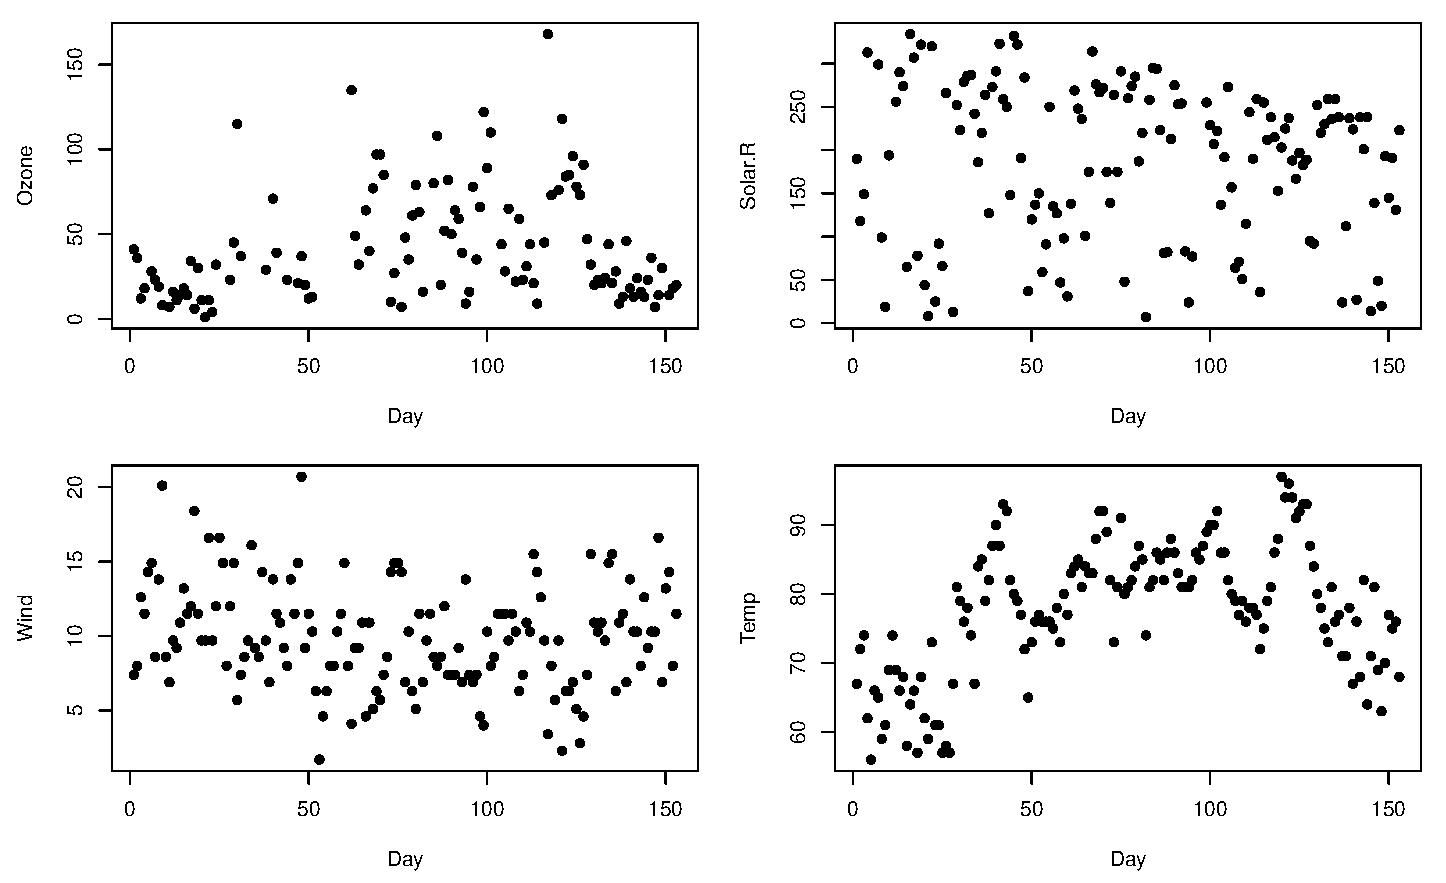
\includegraphics{figures/unnamed-chunk-10-1.pdf}

\hypertarget{tricky-plot-solutions}{%
\subsection*{Tricky plot solutions}\label{tricky-plot-solutions}}
\addcontentsline{toc}{subsection}{Tricky plot solutions}

\texttt{for\ loops} are also useful for plotting data in tricky ways. Let's use a different built-in dataset, that shows the performance of various car make/models.

\begin{verbatim}
                   mpg cyl disp  hp drat    wt  qsec vs am gear carb
Mazda RX4         21.0   6  160 110 3.90 2.620 16.46  0  1    4    4
Mazda RX4 Wag     21.0   6  160 110 3.90 2.875 17.02  0  1    4    4
Datsun 710        22.8   4  108  93 3.85 2.320 18.61  1  1    4    1
Hornet 4 Drive    21.4   6  258 110 3.08 3.215 19.44  1  0    3    1
Hornet Sportabout 18.7   8  360 175 3.15 3.440 17.02  0  0    3    2
Valiant           18.1   6  225 105 2.76 3.460 20.22  1  0    3    1
\end{verbatim}

Let's say we want to see how gas mileage is affected by the number of cylinders a car has. It would be nice to create a plot that shows the raw data as well as the mean mileage for each cylinder number.

\begin{verbatim}
[1] 6 4 8
\end{verbatim}

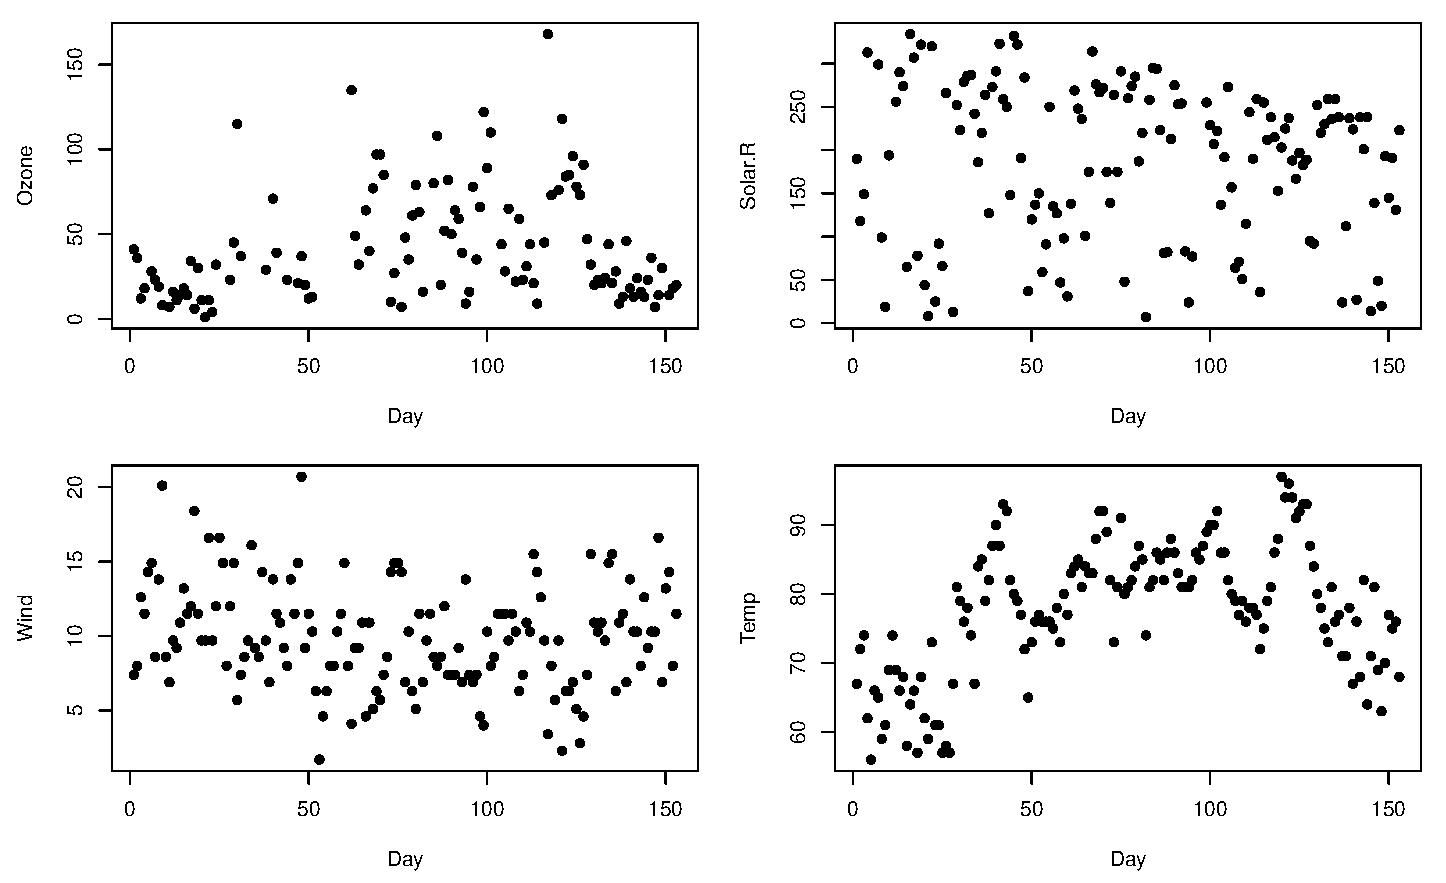
\includegraphics{figures/unnamed-chunk-12-1.pdf}

\hypertarget{exercise-2}{%
\subsection*{Exercise 2}\label{exercise-2}}
\addcontentsline{toc}{subsection}{Exercise 2}

Now try to do something similar on your own with the \texttt{airquality} dataset. Use \texttt{for\ loops} to create a plot with Month on the x axis and Temperature on the y axis. On this plot, depict all the temperatures recorded in each month in the color grey, then superimpose the mean temperature for each month.

We will provide the empty plot, you provide the \texttt{for\ loop}:

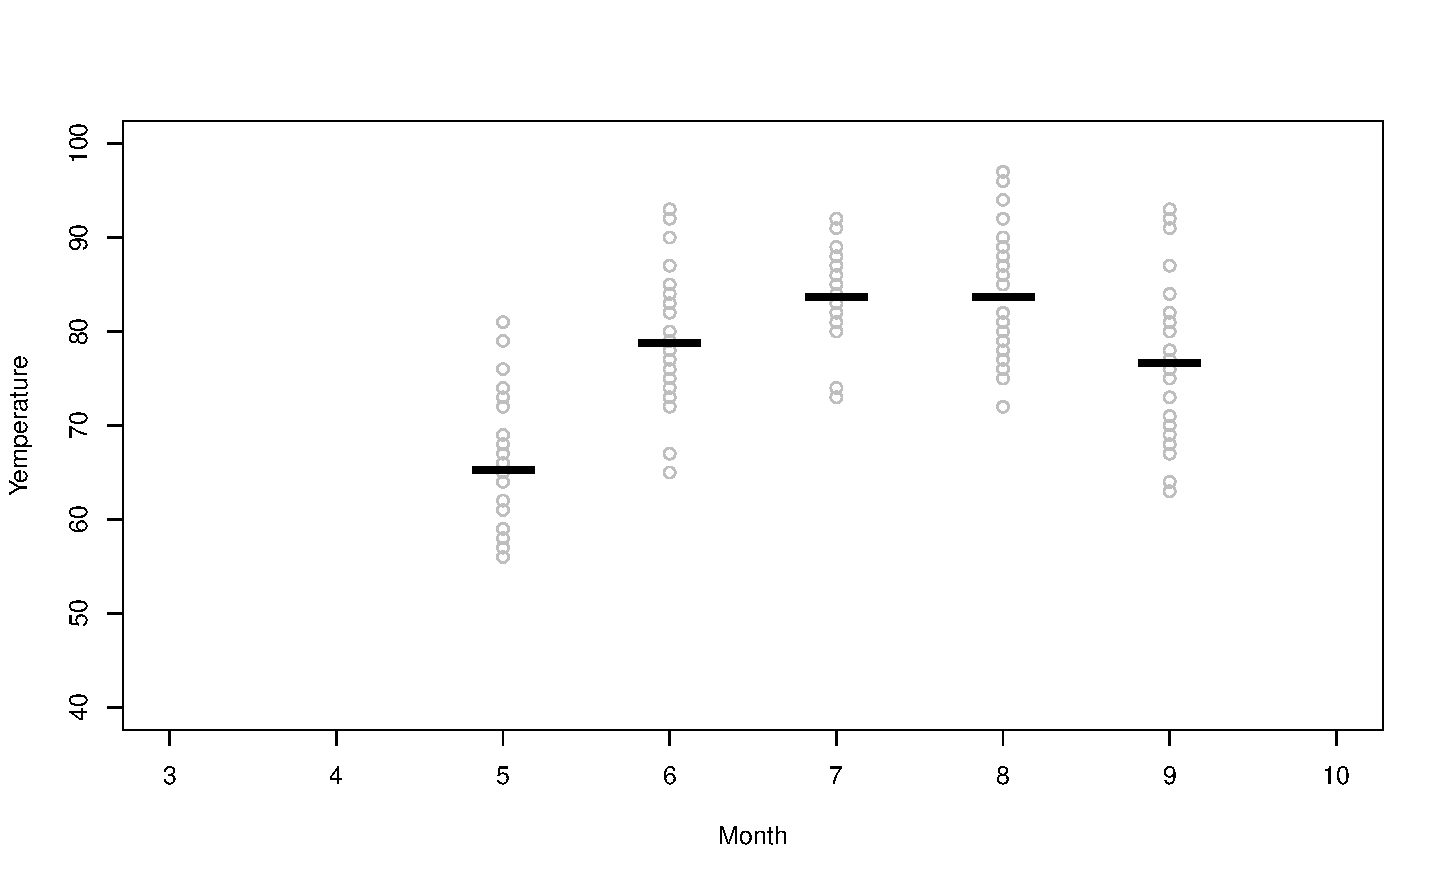
\includegraphics{figures/unnamed-chunk-13-1.pdf}

\hypertarget{using-a-for-loop-with-more-complex-data}{%
\section*{\texorpdfstring{Using a \texttt{for\ loop} with more complex data}{Using a for loop with more complex data}}\label{using-a-for-loop-with-more-complex-data}}
\addcontentsline{toc}{section}{Using a \texttt{for\ loop} with more complex data}

Here's another good example of the power of a good \texttt{for\ loop}.

First, read in some cool data.

\begin{verbatim}
  year month day_of_month day_of_year year_dec frac_of_year    CO2
1 1974     5           26    145.4890 1974.399       0.3986 332.95
2 1974     6            2    152.4970 1974.418       0.4178 332.35
3 1974     6            9    159.5050 1974.437       0.4370 332.20
4 1974     6           16    166.5130 1974.456       0.4562 332.37
5 1974     6           23    173.4845 1974.475       0.4753 331.73
6 1974     6           30    180.4925 1974.495       0.4945 331.68
\end{verbatim}

This is the famous Keeling Curve dataset: long-term monitoring of atmospheric CO2 measured at a volcanic observatory in Hawaii.

Try plotting the Keeling Curve:

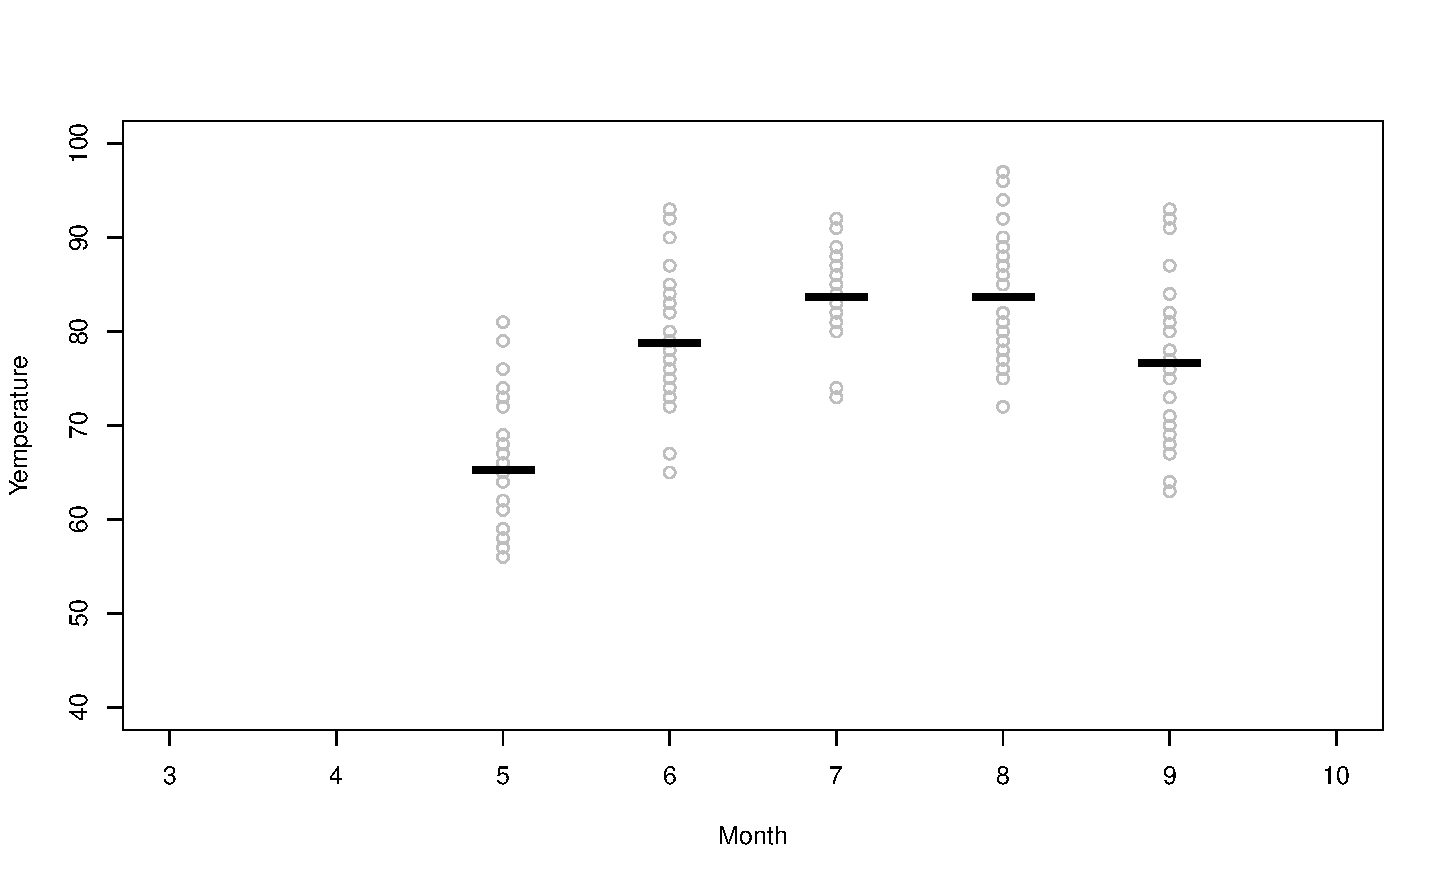
\includegraphics{figures/unnamed-chunk-15-1.pdf}

There are some erroneous data points! We clearly can't have negative CO2 values. Let's remove those and try again:

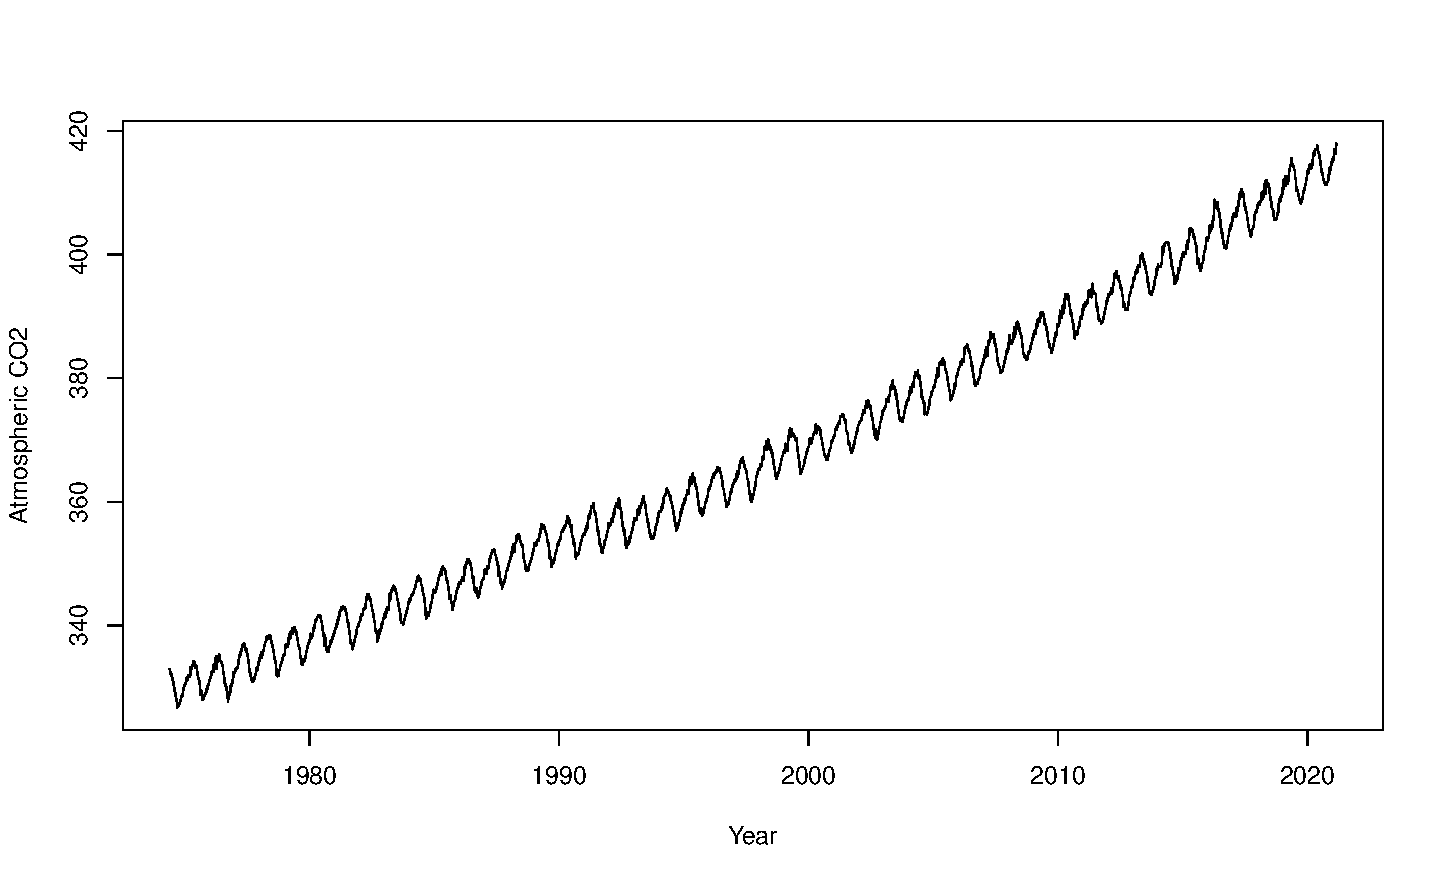
\includegraphics{figures/unnamed-chunk-16-1.pdf}

\textbf{What's the deal with those squiggles?} Let's investigate!

Let's look at the data a different way: \emph{by focusing in on a single year.}

\begin{verbatim}
    year month day_of_month day_of_year year_dec frac_of_year    CO2
816 1990     1            7      6.4970 1990.018       0.0178 353.58
817 1990     1           14     13.5050 1990.037       0.0370 353.99
818 1990     1           21     20.5130 1990.056       0.0562 353.92
819 1990     1           28     27.4845 1990.075       0.0753 354.39
820 1990     2            4     34.4925 1990.094       0.0945 355.04
821 1990     2           11     41.5005 1990.114       0.1137 355.09
\end{verbatim}

\begin{verbatim}
[1] 354.4538
\end{verbatim}

\begin{verbatim}
 [1] -0.87384615 -0.46384615 -0.53384615 -0.06384615  0.58615385  0.63615385
 [7]  0.96615385  0.72615385  1.13615385  1.33615385  1.08615385  1.67615385
[13]  1.81615385  1.71615385  1.77615385  2.41615385  2.50615385  3.24615385
[19]  2.79615385  2.87615385  2.92615385  2.52615385  1.79615385  1.72615385
[25]  1.33615385  1.76615385  0.53615385 -0.16384615 -0.08384615 -0.46384615
[31] -1.28384615 -0.99384615 -1.37384615 -2.65384615 -3.29384615 -3.59384615
[37] -2.70384615 -2.99384615 -3.05384615 -2.91384615 -2.88384615 -2.72384615
[43] -2.05384615 -1.74384615 -1.30384615 -1.00384615 -0.76384615 -0.55384615
[49]  0.01615385 -0.11384615  0.37615385  0.34615385          NA
\end{verbatim}

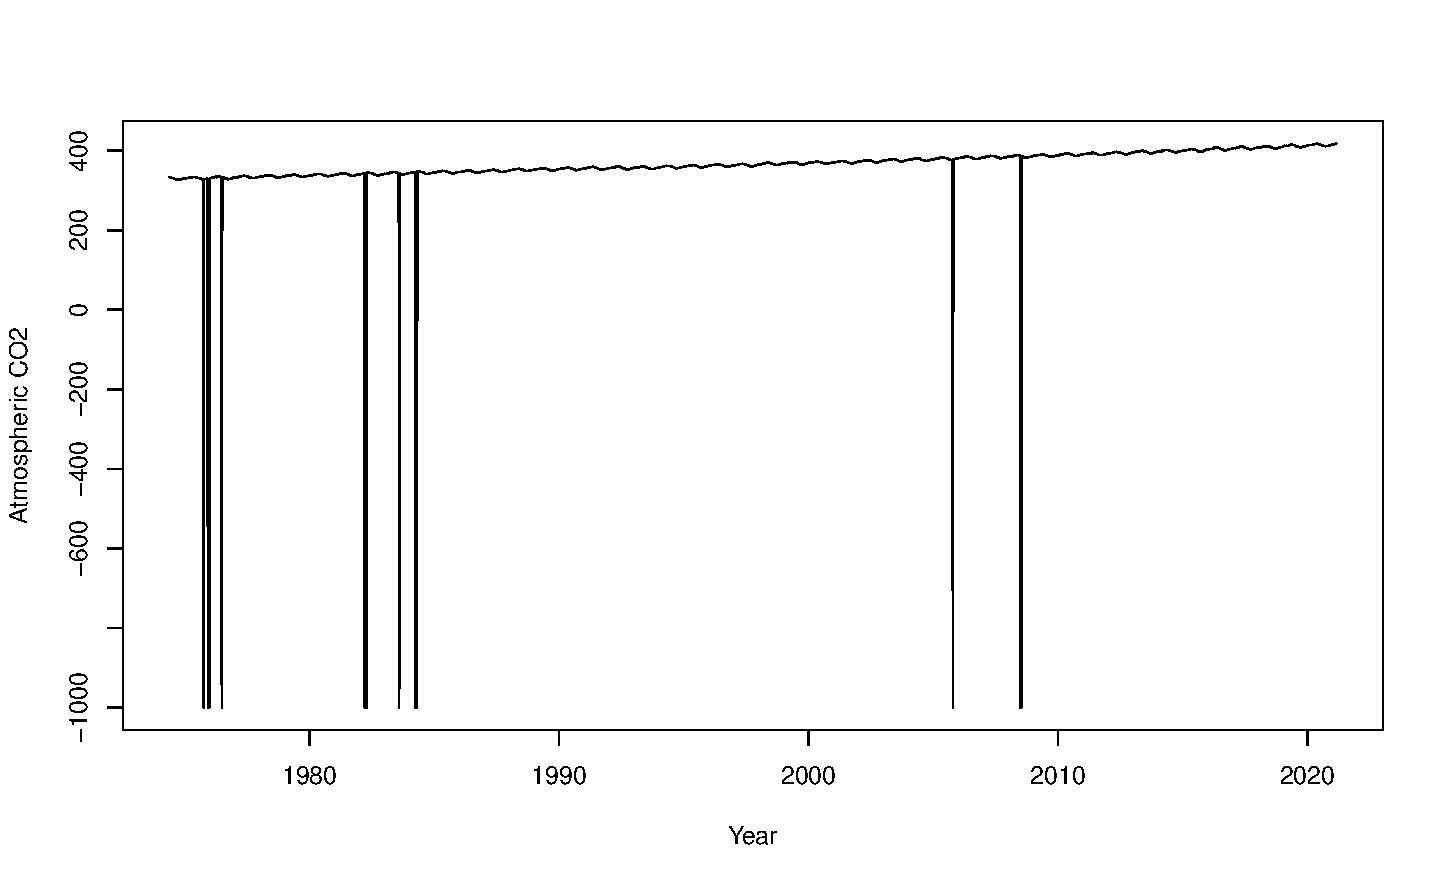
\includegraphics{figures/unnamed-chunk-17-1.pdf}

But this only shows one year of data! How can we include the seasonal squiggle from other years?

Let's use a \texttt{for\ loop}!

OK -- let's redo that graph and add a \texttt{for\ loop} into the mix:

\begin{verbatim}
 [1] "1974" "1975" "1976" "1977" "1978" "1979" "1980" "1981" "1982" "1983"
[11] "1984" "1985" "1986" "1987" "1988" "1989" "1990" "1991" "1992" "1993"
[21] "1994" "1995" "1996" "1997" "1998" "1999" "2000" "2001" "2002" "2003"
[31] "2004" "2005" "2006" "2007" "2008" "2009" "2010" "2011" "2012" "2013"
[41] "2014" "2015" "2016" "2017" "2018" "2019" "2020" "2021" NA    
\end{verbatim}

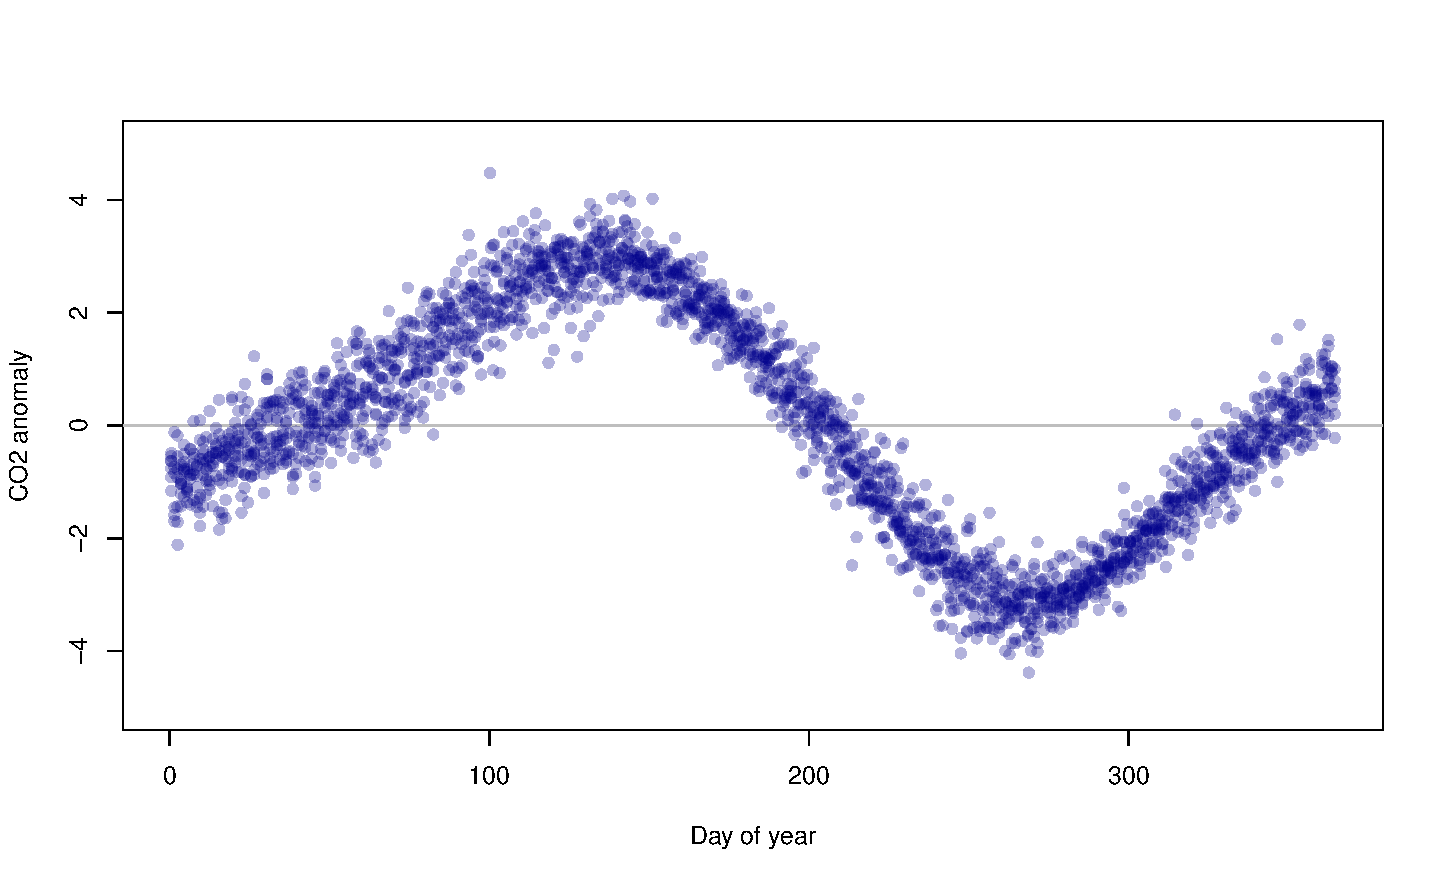
\includegraphics{figures/unnamed-chunk-18-1.pdf}

Beautiful! So how do you interpret this graph? Why does the squiggle happen every year?

\hypertarget{review-assignment}{%
\section*{Review assignment}\label{review-assignment}}
\addcontentsline{toc}{section}{Review assignment}

First, read in and format some other cool data. The code for doing so is provided for you here:

This dataset, freely available from World Bank, shows the renewable electricity output for various countries, presented as a percentage of the nation's total electricity output. They provide this data as a time series.

\hypertarget{summarize-columns-with-a-for-loop}{%
\subsection{\texorpdfstring{Summarize columns with a \texttt{for\ loop}}{Summarize columns with a for loop}}\label{summarize-columns-with-a-for-loop}}

\textbf{Task 1:} Use a \texttt{for\ loop} to find the change in renewable energy output for each nation in the dataset between 1990 and 2015. Print the difference for each nation in the console.

\begin{verbatim}
 [1] "year"           "World"          "Australia"      "Canada"        
 [5] "China"          "Denmark"        "India"          "Japan"         
 [9] "New_Zealand"    "Sweden"         "Switzerland"    "United_Kingdom"
[13] "United_States" 
\end{verbatim}

\begin{verbatim}
[1] "World : 3% change."
[1] "Australia : 4% change."
[1] "Canada : 1% change."
[1] "China : 4% change."
[1] "Denmark : 62% change."
[1] "India : -9% change."
[1] "Japan : 5% change."
[1] "New_Zealand : 0% change."
[1] "Sweden : 12% change."
[1] "Switzerland : 7% change."
[1] "United_Kingdom : 23% change."
[1] "United_States : 2% change."
\end{verbatim}

\textbf{Task 2:} Re-do this loop, but instead of printing the differences to the console, save them in a vector.

\begin{verbatim}
[1] "World : 3% change."
[1] "Australia : 4% change."
[1] "Canada : 1% change."
[1] "China : 4% change."
[1] "Denmark : 62% change."
[1] "India : -9% change."
[1] "Japan : 5% change."
[1] "New_Zealand : 0% change."
[1] "Sweden : 12% change."
[1] "Switzerland : 7% change."
[1] "United_Kingdom : 23% change."
[1] "United_States : 2% change."
\end{verbatim}

\begin{verbatim}
 [1]  3.49241703  3.98181045  0.63273122  3.51887728 62.33064943 -9.14624362
 [7]  4.73004321  0.07524008 12.26263811  7.21543884 23.01128298  1.69994636
\end{verbatim}

\hypertarget{multi-pane-plots-with-for-loops}{%
\subsection*{\texorpdfstring{Multi-pane plots with \texttt{for\ loops}}{Multi-pane plots with for loops}}\label{multi-pane-plots-with-for-loops}}
\addcontentsline{toc}{subsection}{Multi-pane plots with \texttt{for\ loops}}

\hypertarget{practice-with-a-single-plot}{%
\subsection*{Practice with a single plot}\label{practice-with-a-single-plot}}
\addcontentsline{toc}{subsection}{Practice with a single plot}

\textbf{Task 3:} First, get your bearings by figuring out how to use the \texttt{df} dataset to plot the time series for the United States, for the years 1990 - 2015. Label the x axis ``Year'' and the y axis ``\% Renewable''. Include the full name of the county as the \texttt{main} title for the plot.

\begin{verbatim}
  year    World Australia   Canada    China  Denmark    India     Japan
1 1990 19.36204  9.656031 62.37872 20.40794 3.175275 24.48929 11.254738
2 1991 19.23357 10.598201 61.41041 18.47113 2.892325 22.80740 11.856735
3 1992 19.15840 10.066865 61.67921 17.58468 4.398464 20.75265 10.162888
4 1993 19.78795 10.549144 61.72233 18.12526 4.730088 19.55881 11.454528
5 1994 19.53812 10.194474 60.40045 18.08844 4.295431 21.21910  7.993026
6 1995 19.83536  9.624143 61.00410 19.21414 5.035639 17.26054  9.416323
  New_Zealand   Sweden Switzerland United_Kingdom United_States
1    80.00620 51.00011    54.98254       1.828767     11.528647
2    77.18945 44.30088    57.16370       1.656439     10.757414
3    72.58771 52.33321    56.90938       2.005662      9.916110
4    77.02407 52.92433    59.57279       1.777626     10.484326
5    82.05216 43.02873    60.57322       2.139842      9.747236
6    83.85281 47.57878    57.42996       2.066535     10.801085
\end{verbatim}

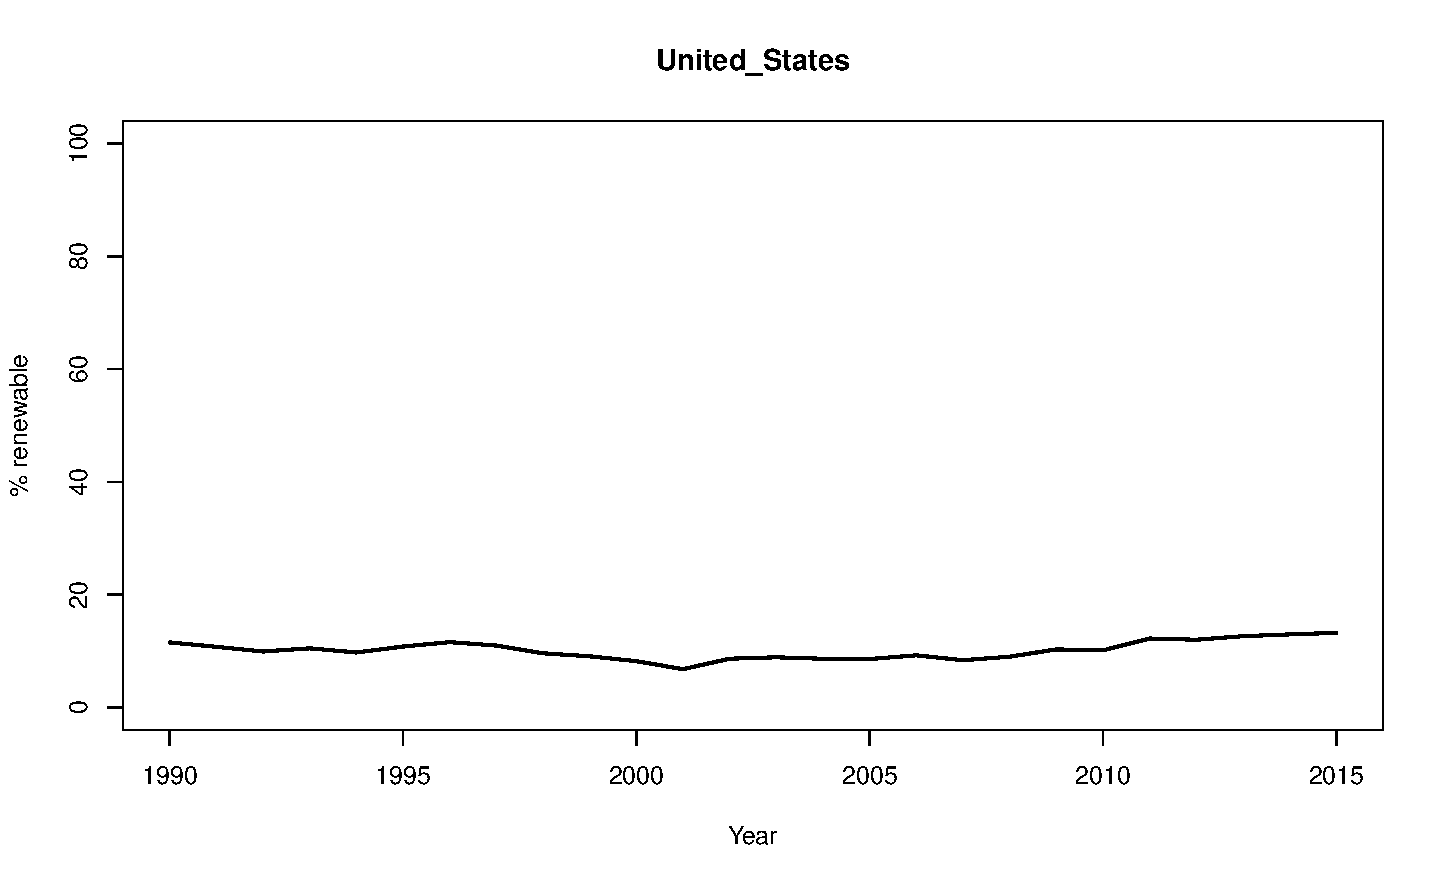
\includegraphics{figures/unnamed-chunk-22-1.pdf}

\hypertarget{now-loop-it}{%
\subsection*{Now loop it!}\label{now-loop-it}}
\addcontentsline{toc}{subsection}{Now loop it!}

\textbf{Task 4:} Use that code as the foundation for building up a \texttt{for\ loop} that displays the same time series for every country in the dataset on a multi-pane graph that with 4 rows and 3 columns.

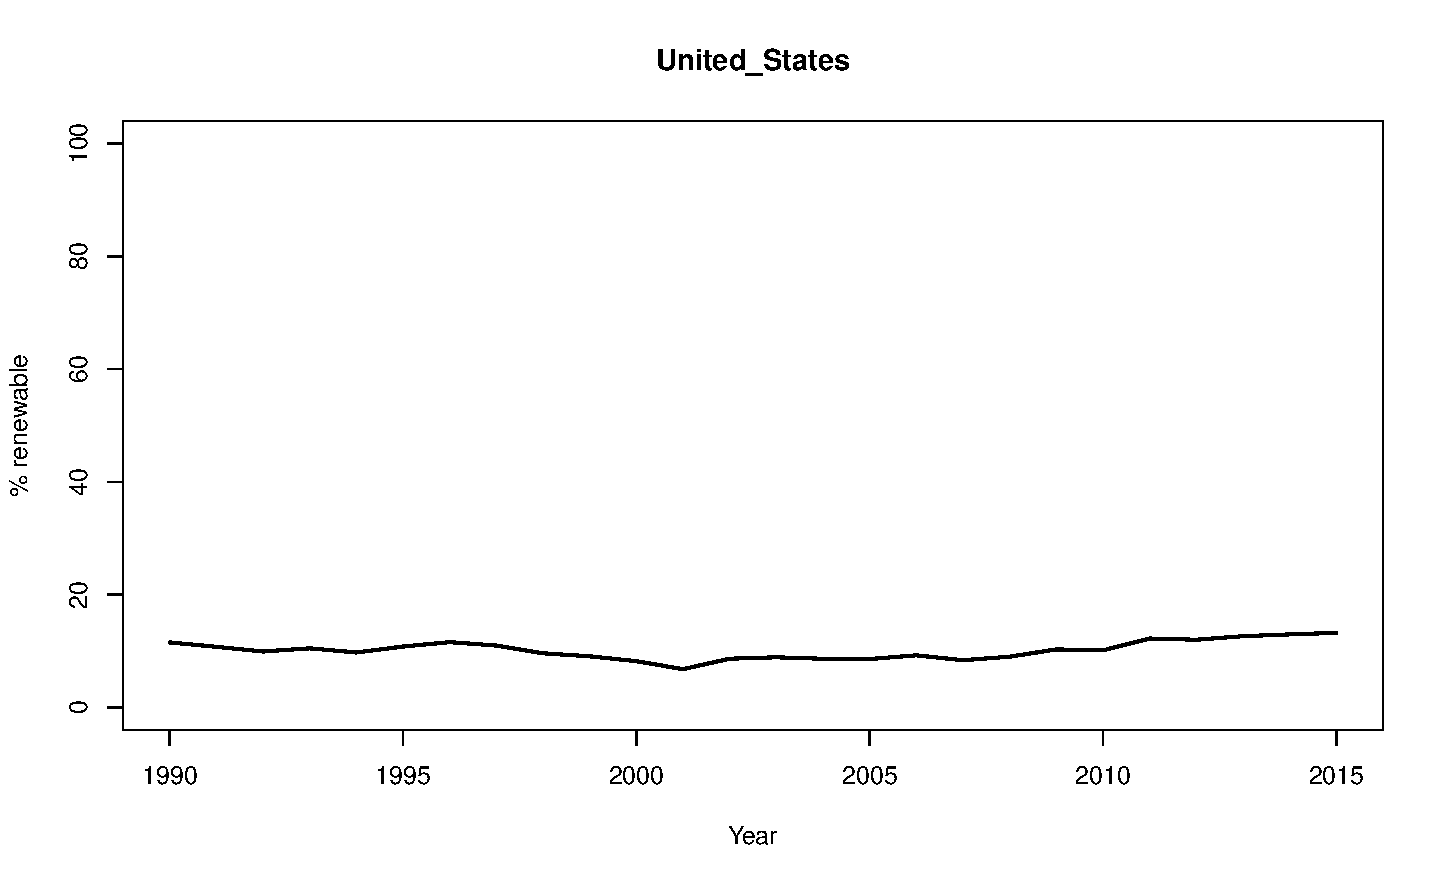
\includegraphics{figures/unnamed-chunk-23-1.pdf}

\hypertarget{now-loop-it-differently}{%
\subsection*{Now loop it differently!}\label{now-loop-it-differently}}
\addcontentsline{toc}{subsection}{Now loop it differently!}

\textbf{Task 5:} Now try a different presentation. Instead of producing 12 different plots, superimpose the time series for each country on the \emph{same single plot}.

To add some flare, highlight the USA curve by coloring it red and making it thicker.

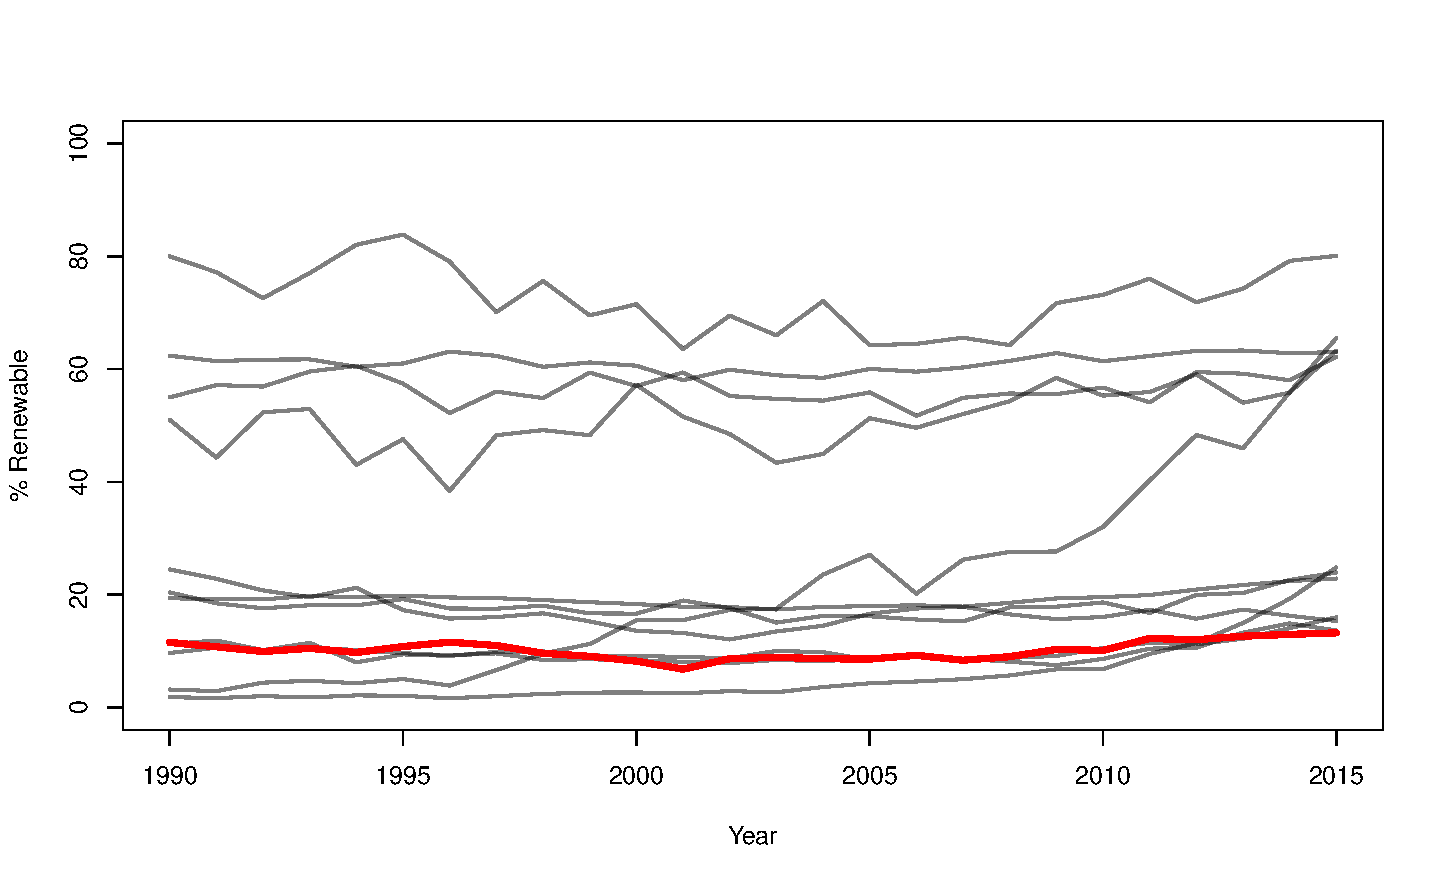
\includegraphics{figures/unnamed-chunk-24-1.pdf}

\hypertarget{writing-functions}{%
\chapter{Writing functions}\label{writing-functions}}

\hypertarget{working-with-text}{%
\chapter{Working with text}\label{working-with-text}}

\hypertarget{working-with-dates-times}{%
\chapter{Working with dates \& times}\label{working-with-dates-times}}

\hypertarget{working-with-factors}{%
\chapter{Working with factors}\label{working-with-factors}}

\hypertarget{cleaning-messy-data}{%
\chapter{Cleaning messy data}\label{cleaning-messy-data}}

\hypertarget{matrices-lists}{%
\chapter{Matrices \& lists}\label{matrices-lists}}

\hypertarget{pipes}{%
\chapter{Pipes}\label{pipes}}

\hypertarget{exporting-data-plots}{%
\chapter{Exporting data \& plots}\label{exporting-data-plots}}

\hypertarget{part-interactive-dashboards}{%
\part{Interactive dashboards}\label{part-interactive-dashboards}}

\hypertarget{intro-to-shiny-apps}{%
\chapter{Intro to Shiny apps}\label{intro-to-shiny-apps}}

\hypertarget{shiny-dashboards}{%
\chapter{Shiny dashboards}\label{shiny-dashboards}}

\hypertarget{data-entry-apps}{%
\chapter{Data entry apps}\label{data-entry-apps}}

\hypertarget{part-databases}{%
\part{Databases}\label{part-databases}}

\hypertarget{introduction}{%
\chapter{Introduction}\label{introduction}}

\hypertarget{what}{%
\section{What}\label{what}}

\hypertarget{why}{%
\section{Why}\label{why}}

\hypertarget{when}{%
\section{When}\label{when}}

\hypertarget{when-not}{%
\section{When not}\label{when-not}}

\hypertarget{platforms}{%
\chapter{Platforms}\label{platforms}}

\hypertarget{postgresql}{%
\section{PostgreSQL}\label{postgresql}}

\hypertarget{mysql}{%
\section{mySQL}\label{mysql}}

\hypertarget{sqlite}{%
\section{SQLite}\label{sqlite}}

\hypertarget{alternatives}{%
\chapter{Alternatives}\label{alternatives}}

\hypertarget{nosql}{%
\section{NoSQL}\label{nosql}}

\hypertarget{practices}{%
\chapter{Practices}\label{practices}}

Spinning up a local DB

\hypertarget{part-documenting-your-work}{%
\part{Documenting your work}\label{part-documenting-your-work}}

\hypertarget{r-markdown}{%
\chapter{R Markdown}\label{r-markdown}}

\hypertarget{reproducible-research}{%
\chapter{Reproducible research}\label{reproducible-research}}

\hypertarget{automated-reporting}{%
\chapter{Automated reporting}\label{automated-reporting}}

\hypertarget{formatting-standards}{%
\chapter{Formatting standards}\label{formatting-standards}}

\hypertarget{tables-1}{%
\section{Tables}\label{tables-1}}

\hypertarget{figures}{%
\section{Figures}\label{figures}}

\hypertarget{captions}{%
\section{Captions}\label{captions}}

\hypertarget{part-version-control-and-teamwork}{%
\part{Version control and teamwork}\label{part-version-control-and-teamwork}}

\hypertarget{what-is-version-control}{%
\chapter{What is version control?}\label{what-is-version-control}}

\hypertarget{what-is-git}{%
\chapter{What is Git?}\label{what-is-git}}

\hypertarget{repositories}{%
\section{Repositories}\label{repositories}}

\hypertarget{github}{%
\section{Github}\label{github}}

\hypertarget{standard-git-operations}{%
\chapter{Standard git operations}\label{standard-git-operations}}

\hypertarget{a-git-workflow}{%
\chapter{A git workflow}\label{a-git-workflow}}

\hypertarget{other-git-platforms}{%
\chapter{Other git platforms}\label{other-git-platforms}}

\hypertarget{part-writing-about-data}{%
\part{Writing about data}\label{part-writing-about-data}}

\hypertarget{types-of-writing}{%
\chapter{Types of writing}\label{types-of-writing}}

\hypertarget{grant-proposals}{%
\section{Grant proposals}\label{grant-proposals}}

\hypertarget{reports-and-publications}{%
\section{Reports and publications}\label{reports-and-publications}}

\hypertarget{fundraising}{%
\section{Fundraising}\label{fundraising}}

\hypertarget{press-releases}{%
\section{Press releases}\label{press-releases}}

\hypertarget{elements-of-style}{%
\chapter{Elements of style}\label{elements-of-style}}

\hypertarget{sections-of-a-report}{%
\chapter{Sections of a report}\label{sections-of-a-report}}

\hypertarget{abstract}{%
\section{Abstract}\label{abstract}}

\hypertarget{introduction-1}{%
\section{Introduction}\label{introduction-1}}

\hypertarget{methods}{%
\section{Methods}\label{methods}}

\hypertarget{results}{%
\section{Results}\label{results}}

\hypertarget{discussion}{%
\section{Discussion}\label{discussion}}

\hypertarget{other-elements}{%
\section{Other elements}\label{other-elements}}

\hypertarget{acknowledgments}{%
\subsection{Acknowledgments}\label{acknowledgments}}

\hypertarget{literature-cited}{%
\subsection{Literature Cited}\label{literature-cited}}

\hypertarget{tables-2}{%
\subsection{Tables}\label{tables-2}}

\hypertarget{figures-1}{%
\subsection{Figures}\label{figures-1}}

\hypertarget{supplementary-materials}{%
\subsection{Supplementary Materials}\label{supplementary-materials}}

\hypertarget{part-creating-websites}{%
\part{Creating websites}\label{part-creating-websites}}

\hypertarget{part-advanced-skills}{%
\part{Advanced skills}\label{part-advanced-skills}}

\hypertarget{mapping}{%
\chapter{Mapping}\label{mapping}}

\hypertarget{geographic-computing-gis}{%
\chapter{Geographic computing \& GIS}\label{geographic-computing-gis}}

\hypertarget{statistical-modeling}{%
\chapter{Statistical modeling}\label{statistical-modeling}}

\hypertarget{apply-family}{%
\chapter{Apply family}\label{apply-family}}

\hypertarget{iterative-statistics}{%
\chapter{Iterative statistics}\label{iterative-statistics}}

\hypertarget{iterative-simulations}{%
\chapter{Iterative simulations}\label{iterative-simulations}}

\hypertarget{image-analysis}{%
\chapter{Image analysis}\label{image-analysis}}

\hypertarget{machine-learning}{%
\chapter{Machine learning}\label{machine-learning}}

  \bibliography{book.bib,packages.bib}

\end{document}
